\documentclass[a4paper,dvipdfmx]{jsarticle}
\usepackage{graphicx}
\usepackage{fancybox}
\usepackage{ascmac}
\usepackage{amsmath}
\usepackage{amsfonts}
\usepackage{comment}
\usepackage{here}
\usepackage{listings,jlisting}
\usepackage[a4paper,margin=2cm,truedimen]{geometry}
\usepackage{amssymb}
\usepackage[svgnames]{xcolor}

  \definecolor{diffstart}{named}{Grey}
  \definecolor{diffincl}{named}{Green}
  \definecolor{diffrem}{named}{OrangeRed}

  \lstdefinelanguage{diff}{
    basicstyle=\ttfamily\small,
    morecomment=[f][\color{diffstart}]{@@},
    morecomment=[f][\color{diffincl}]{+\ },
    morecomment=[f][\color{diffrem}]{-\ },
  }

\newcommand{\image}[3]{
    \begin{figure}[H]
        \begin{center}
        \includegraphics[bb=0 0 480 360,width=14cm]{#2}
        \end{center}
        \caption{#1}
        \label{#3}
    \end{figure}
}

\lstset{
	%language=[Objective]Caml,
	language=Python,
    basicstyle=\ttfamily,
    keywordstyle=\color[RGB]{33,74,180}\bfseries,
    stringstyle=\color[RGB]{240,100,5},
    commentstyle=\color[RGB]{100,100,100}\itshape,
    numberstyle=\footnotesize,
    numbers=left,
    stepnumber=1,
    numbersep=15pt,
    backgroundcolor=\color[RGB]{251,251,251},
    frame=single,
    frameround=ffff,
    framesep=5pt,
    rulecolor=\color[RGB]{128,128,128}, 
    breaklines=true,
    breakautoindent=true,
    breakatwhitespace=true,
    breakindent=25pt,
    showspaces=false,
    showstringspaces=false,
    showtabs=false,
    tabsize=2,
    captionpos=b,
    linewidth=\textwidth,
}
%\end{comment}
\begin{document}
% タイトルはここ
%\title{機能設計仕様書}
% 自分の情報はここに
%\author{工学部情報学科計算機科学コース \\ 1029-28-8969 渡邊 綾仁}

% 提出日って書いているけどコンパイルした日
% 使いたくなかったらコメントアウト

% \date{提出日: \today}

%\maketitle

% 以下、コピペ用
% includegraphicsとかtableとかめんどくさいのでここに書いておくとよさそう

\begin{comment}
%コメントアウトここから
% ----------------

%画像挿入用
\begin{figure}[H]
\begin{center}
\includegraphics[width=14cm]{hoge.png}
\end{center}
\caption{キャプション}
\label{参照ラベル}
\end{figure}

%ソースコード挿入用
\begin{lstlisting}[basicstyle=\ttfamily\footnotesize, frame=single]
\end{lstlisting}

%table環境
\begin{table}[H]
\begin{center}
\caption{キャプション}
  \begin{tabular}{|c|c|c|c|} \hline
    ノード名 & 割り当てたピンの番号 & 信号名 & スイッチ名 \\ \hline \hline
  \end{tabular}
	\label{ラベル}
\end{center}
\end{table}


%コメントアウトおしまい
\end{comment}

%20180506 メモ
\begin{comment}
simple.pdfのSIMPLE/Bの記述が、方式設計レベルの仕様書に該当するようなので、
このような記述方法を参考にすると、多分system_design_spec.pdfは書きやすいかも。
\end{comment}
%メモおしまい

% ----------------
%ここから本文
\section*{課題4}

\subsection*{課題内容}

MNIST のテスト画像1 枚を入力とし,3 層ニューラルネットワークを用いて,0~9 の値のうち1 つを出力するプログラムを作成せよ.

\subsection*{作成したプログラムについて}

課題1 で作成した my\_nn\_test.py に改良を加えた。
課題1から追加、変更になった点は以下の通りである。

\begin{itemize}
	\item 課題2, 3において作成した、学習後のパラメータを記録したファイルを読み込み、識別を行う
	\item 標準入力から不正な値が入力された場合、ファイルが存在しなかった場合などの例外処理
\end{itemize}

\begin{enumerate}
	\item NNTest クラスインスタンスの作成
	\item 学習したパラメータを利用して識別を行う場合は、ファイル名を標準入力から入力、課題1のようにランダムに初期化されたパラメータを用いて識別を行う場合は何も入力せずに進む。ファイルが存在しない場合はエラーとする。\\
	・パラメータをファイルから読み込んだ場合
	\begin{enumerate}
		\item パラメータをファイルから読み込んだ場合は、インスタンス作成時に初期化した各パラメータを読み込んだパラメータに書き換える。
		\item 中間層の活性化関数をシグモイド関数、ReLU、Dropout、ReLU + Batch normalization からパラメータファイルの内容に応じて選択する。 
		\item テスト回数を1〜1000の間で設定する。ここでテスト回数を1に設定すると、課題4の仕様の通り、画像1枚を入力(0〜9999の整数を1つ入力)として識別を行い、正解ラベルと認識結果を標準出力に出力する。
		\item テスト回数が2回以上の場合は、テストデータ10000枚の画像から1回あたり100枚の画像をランダムに選んで識別を行い、Accuracy を計算する。終了後、テスト回数とAccuracy の関係のグラフを出力し、標準出力に最終的なAccuracy の値を出力する。
	\end{enumerate}
	・パラメータを読み込まなかった場合
	\begin{enumerate}
		\item 0以上9999以下の整数を標準入力から1つ受け取る。
		\item ランダムに初期化されたパラメータを用いて識別を行い、正解ラベルと認識結果を標準出力に出力する。
	\end{enumerate}
\end{enumerate}


\subsection*{実行結果}

my\_nn\_test.py において、課題3で中間層の活性化関数をシグモイド関数にして 30エポック学習させたパラメータを保存したファイル param\_30epoch.npz を標準入力から読み込ませ、(中間層の活性化関数をシグモイド関数、テスト回数を1としたうえで)0以上9999以下の値を何度か適当に選び、出力結果を確認した。

入力した整数と正解ラベル、および識別器の識別結果をまとめたものを以下の表 \ref{R1-1} に示す。

\begin{table}[H]
\begin{center}
\caption{入力と識別結果の一部}
  \begin{tabular}{|c|c|c|} \hline
    入力値 & 正解ラベル & 認識結果  \\ \hline \hline
    0 & 7 & 7 \\ \hline
    334 & 3 & 3 \\ \hline
    777 & 1 & 1 \\ \hline
    1000 & 9 & 9 \\ \hline
    1729 & 1 & 1 \\ \hline
    4126 & 8 & 8 \\ \hline
    5887 & 7 & 0 \\ \hline
    9999 & 6 & 6 \\ \hline
  \end{tabular}
	\label{R1-1}
\end{center}
\end{table}

また、MNIST テストデータ10000枚を用いて、バッチサイズ100、テスト回数1000回に設定してテストを行ったところ、認識精度は 91.11\% となっており、パラメータがうまく学習できていることが確認できた。

\subsection*{工夫点、問題点}
誰がプログラムを実行してもスムーズに進められるように、メッセージを充実させたり、認識結果と正解ラベルと画像を表示することによって、正しい識別が行われたかどうかを確認しやすくしたりしている。また、発展課題で行った実装のテストも行いやすいように汎用性を高めている。

\newpage

\section*{発展課題の実装内容}

\subsection*{A1: ReLU}

\subsubsection*{実装内容}

my\_nn\_learn.py, my\_nn\_test.py にReLU 関数を定義した。
ReLU 関数の順伝播の定義は、以下のソースコード \ref{A1-1} のようになっている。

\begin{lstlisting}[caption="ReLU 関数(順伝播)",label=A1-1]
def relu_forward(t):
    return np.maximum(t, 0)
\end{lstlisting}

これは、$t$ と $0$ のうち大きい方を返すように実装している。

また、ReLU の逆伝播を行う関数については以下のソースコード \ref{A1-2} のようになっている。

\begin{lstlisting}[caption="ReLU 関数(逆伝播)",label=A1-2]
def relu_backward(t):
    return np.where(t > 0, 1, 0)
\end{lstlisting}

順伝播で $t > 0$ となっている要素に対しては1, それ以外に対しては 0 を返す実装になっている。\\

必須課題においては中間層の活性化関数にシグモイド関数を用いていたが、この活性化関数を ReLU 関数に置き換えられるように my\_nn\_learn.py を実行した時に選択できるようにした。また、逆伝播についても、順伝播でReLUを用いた時は、ReLU 関数の微分に置き換えられる。ReLUの逆伝播を行っている部分は、my\_nn\_learn.py の 540 行目にあたり、以下のソースコード \ref{A1-3} のようになっている。

\begin{lstlisting}[caption="ReLU の逆伝播 を行う部分",label=A1-3]
bp_data['g_activate_mid'] = np.dot(nn.network['w2'].T, bp_data['g_en_ak']) * relu_backward(data['a1'])
\end{lstlisting}

\subsubsection*{実行結果}

バッチサイズ $100$、学習係数 $0.01$、エポック数 $30$ 、最適化手法をSGDにし、活性化関数をシグモイド関数にしたものとReLU関数に設定したものをそれぞれ学習させた。なお、活性化関数をシグモイド関数にしたものは param\_sigmoid\_sgd\_30.npz、ReLU関数を用いたものは param\_relu\_sgd\_30.npz として提出したファイルに含めている。横軸に学習回数、縦軸にクロスエントロピー誤差の平均値をとったグラフを作成したところ、以下の図 \ref{fig-A-1-1} のようになった。

\image{ReLUとシグモイド関数の比較}{report_a1-1.png}{fig-A-1-1}

図 \ref{fig-A-1-1} の青い線がシグモイド関数を用いた時のクロスエントロピー誤差の平均値の値、橙色の線がReLU関数を用いた時の値である。図 \ref{fig-A-1-1} からReLU関数を用いた時も正しく学習が進んでいることと、シグモイド関数を用いた時よりも学習が早く、また学習用データに対しての認識精度もシグモイド関数を用いた時より上がっていることがわかる。

また、テストデータを用いて、param\_sigmoid\_sgd\_30.npz、param\_relu\_sgd\_30.npz のそれぞれに対して100回テストを行ったところ認識精度は以下の表 \ref{table-A1-1} のようになった。

\begin{table}[H]
\begin{center}
\caption{テストデータでの認識精度(活性化関数の比較)}
  \begin{tabular}{|c|c|} \hline
    活性化関数 & 認識精度  \\ \hline \hline
    シグモイド & 91.052 \%  \\ \hline
    ReLU & 95.12 \% \\ \hline
  \end{tabular}
	\label{table-A1-1}
\end{center}
\end{table}

表 \ref{table-A1-1} から、ReLU関数の方がシグモイド関数を用いるより認識精度が高く、汎化性能が高いことがわかる。

\subsection*{A2: Dropout}

\subsubsection*{実装内容}

my\_nn\_learn.py, my\_nn\_test.py に Dropout を行うためのクラス Dropout を定義した。
学習時における Dropout クラスは my\_nn\_learn.py の79行目から定義されており、以下のソースコード \ref{A2-1} のようになっている。

\begin{lstlisting}[caption="クラス Dropout ",label=A2-1]
class Dropout:
    """ Class of Dropout

    Attributes:
        dropout_num: the node numbers that don't propagate the signal.
        mask: the mask of dropout.

    """
    # the rate of dropout
    rho = 0.5

    def __init__(self, nn):
        """ Initialize Dropout Class """
        self.dropout_num = np.random.choice(nn.m, int(nn.m * self.rho), replace=False)
        self.mask = np.zeros((nn.m, nn.batch_size))

    def gen_mask(self, nn):
        """ generating mask """
        tmp1 = np.identity(nn.m)[self.dropout_num]
        tmp2 = np.sum(tmp1, axis=0)
        tmp3 = np.repeat(tmp2, nn.batch_size)
        tmp4 = tmp3.reshape((nn.m, nn.batch_size))
        return 1 - tmp4

    def forward(self, nn, t):
        """ forwarding in Dropout """
        self.mask = self.gen_mask(nn)
        return t * self.mask

    def backward(self):
        """ back propagation in Dropout """
        return self.mask
\end{lstlisting}

ソースコード \ref{A2-1} の10行目の rho はパラメータであり、順伝播で無視するノードの割合($ 0 < \rho < 1$)である。変数 nn.m は NNLearn クラスの変数で、中間層のノード数を表しており、nn.batch\_size はバッチサイズを表している。変数  dropout\_num は中間層のノード 0番〜 (nn.m)-1 番のうち伝搬しないノードの番号の値を格納している。mask は順伝播、逆伝播で用いるマスクであり、(nn.m) 行 
 (nn.batch\_size) 列の行列で、中間層において伝播しないノードの行は全て0、他は1となっている。順伝播の時はこのマスクと affine レイヤーからの入力のアダマール積を取ることによって活性化レイヤーに信号を伝播するかしないかを決定しており、逆伝播のときはこのマスク自体を微分した値として伝える。\\
 
 テスト時には、my\_nn\_test.py の221 行目にあるように、全てのノードを伝播するかわりに $1-\rho$ をかけている。
 
 \subsubsection*{実行結果}
 
バッチサイズ $100$、学習係数 $0.01$、エポック数 $30$ 、最適化手法をSGDにし、活性化関数をReLU関数にしたもの(ファイル名: param\_relu\_sgd\_30.npz )とDropout に設定したもの(ファイル名: param\_dropout\_sgd\_30.npz )をそれぞれ学習させた。なおDropout において、無視するノードの割合であるパラメータ$\rho$は$\rho = 0.3$とした。横軸にエポック数、縦軸に認識精度 (Accuracy) をとったグラフを作成したところ、以下の図 \ref{fig-A-2-1} のようになった。

\image{ReLU関数とDropout の比較}{report_a2-1.png}{fig-A-2-1}

図 \ref{fig-A-2-1} の青い線がReLU関数を用いた時の Accuracy 、橙色の線がDropoutを用いた時の値である。図 \ref{fig-A-2-1} から Dropout を用いた時の方が訓練データに対しての認識精度が落ちていることがわかる。

また、テストデータを用いて、param\_relu\_sgd\_30.npz、param\_dropout\_sgd\_30.npz のそれぞれに対して100回テストを行ったところ認識精度は以下の表 \ref{table-A2-1} のようになった。

\begin{table}[H]
\begin{center}
\caption{認識精度(ReLU と Dropout の比較)}
  \begin{tabular}{|c|c|c|c|} \hline
    活性化関数 & 認識精度(訓練データ) & 認識精度(テストデータ)& 差  \\ \hline \hline
    ReLU & 91.783 \% & 95.12 \% & 3.337 \% \\ \hline
    Dropout & 88.692 \% & 91.88 \% &  3.188 \% \\ \hline
  \end{tabular}
	\label{table-A2-1}
\end{center}
\end{table}

表 \ref{table-A2-1} から、Dropout の方が訓練データとテストデータの間の認識精度の差がわずかに小さいが、大きな差はみられなかった。
ネットワーク自体の層が深くはないため、結果にあまり差が出なかったと考えられる。
 
 \subsection*{A3: Batch Normalization}
 
 \subsubsection*{実装内容}
 
 学習用のファイル my\_nn\_learn.py とテスト用のファイル my\_nn\_test.py に BatchNormalization というクラスを作成した。\\
 
 はじめに、学習用のファイル my\_nn\_learn.py の実装内容について説明する。
 
 パラメータやクラス変数の初期化部分は以下のソースコード \ref{A3-1} のようになっている。
 \begin{lstlisting}[caption="Batch Normalization (学習用: 初期化)",label=A3-1]
 class BatchNormalization:

...

    def __init__(self, nn: NNLearn):
        """ Initialize BatchNormalization class """
        self.gamma = 1
        self.beta = 0
        self.x_hat = 0
        self.avg = np.zeros((nn.batch_size, 1))
        self.var = np.zeros((nn.batch_size, 1))
        self.avg_sum = np.zeros(nn.m)
        self.var_sum = np.zeros(nn.m)
        self.epsilon = 10 ** (-8)
\end{lstlisting}

パラメータ gamma, beta は電子テキストのそれぞれ $\gamma, \beta$ に対応している。また、x\_hat, avg, var, epsilon はそれぞれ$\hat{x}, \mu_B, \sigma_B^2, \epsilon$に対応しており、avg\_sum, var\_sum は、それぞれテスト用ファイルで用いる $\mu$の期待値、$\sigma^2$の期待値である。\\

次に、学習用ファイルの順伝播部分の実装について説明する。順伝播の実装内容は以下のソースコード \ref{A3-2}の通りである。また、Batch Normalization の順伝播の計算式も以下に示す。

\begin{eqnarray}
\label{bn1-1}
	\mu_B & \leftarrow & \frac{1}{B} \sum_{i=1}^{B}{x_i} \\
\label{bn1-2}
	\sigma_B^2 & \leftarrow & \frac{1}{B} \sum_{i=1}^{B}{(x_i - \mu_B)^2} \\
\label{bn1-3}
	\hat{x_i} & \leftarrow &  \frac{x_i - \mu_B}{\sqrt{\sigma_B^2 + \epsilon}}\\
\label{bn1-4}
	y_i & \leftarrow & \gamma \hat{x_i} + \beta 
\end{eqnarray}


\begin{lstlisting}[caption="Batch Normalization (学習用: 順伝播)",label=A3-2]
    def forward(self, x: ndarray):
        """ forwarding in Batch normalization """
        self.avg = np.apply_along_axis(np.average, axis=1, arr=x)
        self.avg_sum += self.avg
        self.var = np.apply_along_axis(np.var, axis=1, arr=x)
        self.var_sum += self.var
        self.x_hat = np.apply_along_axis(self.f_normalize, axis=0, arr=x)
        tmp_r = np.apply_along_axis(self.mult_and_move, axis=0, arr=self.x_hat)
        return tmp_r

    def f_normalize(self, t: ndarray):
        """ normalize the array """
        return (t - self.avg) / np.sqrt(self.var + self.epsilon)

    def mult_and_move(self, t: ndarray):
        """ multiplication and movement """
        return self.gamma * t + self.beta
\end{lstlisting}

ソースコード\ref{A3-2}の3行目が式(\ref{bn1-1})、5行目が式(\ref{bn1-2})、7行目が式(\ref{bn1-3})、8行目が式(\ref{bn1-4})に対応している。ソースコード\ref{A3-2}の7行目では$\hat{x_i}$ の正規化を行なっており、この際に 11〜13行目の f\_normalize 関数を用いている。また、ソースコード\ref{A3-2} の8行目で $y_i$ を求めているが、この際に15〜17行目の mult\_and\_move 関数を用いている。\\

次に、学習用ファイルの逆伝播の部分について説明する。逆伝播の実装内容は以下のソースコード \ref{A3-3}の通りである。また、Batch Normalization の逆伝播の計算式も以下に示す。

\begin{eqnarray}
\label{bn2-1}
	\frac{\partial E_n}{\partial \hat{x_i}} & = & \frac{\partial E_n}{\partial \hat{y_i}} \cdot \gamma \\
\label{bn2-2}
	\frac{\partial E_n}{\partial \sigma_B^2} & = & \sum_{i=1}^{B}{\frac{\partial E_n}{\partial \hat{x_i}}} \cdot (\hat{x_i} - \mu_B) \cdot \frac{-1}{2}(\sigma_B^2 + \epsilon)^{\frac{-3}{2}} \\
\label{bn2-3}
	\frac{\partial E_n}{\partial \mu_B} & = & (\sum_{i=1}^{B}{\frac{\partial E_n}{\partial \hat{x_i}} 
	\cdot \frac{-1}{\sqrt{\sigma_B^2 + \epsilon}}) + \frac{\partial E_n}{\partial \sigma_B^2}} \cdot \frac{-2}{B} \sum_{i=1}^{B}{(x_i - \mu_B)} \\
\label{bn2-4}
	\frac{\partial E_n}{\partial x_i} & = & \frac{\partial E_n}{\partial \hat{x_i}} \cdot \frac{1}{\sqrt{\sigma_B^2 + \epsilon}} + \frac{\partial E_n}{\partial \sigma_B^2} \cdot \frac{2(x_i -\mu_B)}{m} + \frac{\partial E_n}{\partial \mu_B} \cdot \frac{1}{B} \\
\label{bn2-5}
	\frac{\partial E_n}{\partial \gamma} & = & \sum_{i=1}^{B}{\frac{\partial E_n}{\partial y_i} \cdot \hat{x_i}} \\
\label{bn2-6}
	\frac{\partial E_n}{\partial \beta} & = & \sum_{i=1}^{B}{\frac{\partial E_n}{\partial y_i}}
\end{eqnarray}

\begin{lstlisting}[caption="Batch Normalization (学習用: 逆伝播)",label=A3-3]
def backward(self, y: ndarray, nn: NNLearn, f_data: dict):
    """ back propagation in Batch normalization """
    d_en_xhati = np.apply_along_axis(lambda l: l * self.gamma, axis=0, arr=y)
    d_en_var = np.sum(d_en_xhati * np.apply_along_axis(lambda l: l - self.avg, axis=0, arr=f_data['a1']), axis=1) \
               / (-2 * (self.var + self.epsilon) ** (3 / 2))
    d_en_mub = np.sum(d_en_xhati, axis=1) / -np.sqrt(self.var + self.epsilon) + (-2 / nn.batch_size) * \
               d_en_var * np.sum(np.apply_along_axis(lambda l: l - self.avg, axis=0, arr=f_data['a1']), axis=1)
    tmp = np.apply_along_axis(lambda l: 2 * d_en_var * (l - self.avg), axis=0, arr=f_data['a1'])
    d_en_xi = np.apply_along_axis(lambda l: l / np.sqrt(self.var + self.epsilon), axis=0, arr=d_en_xhati) + \
              np.apply_along_axis(lambda l: (l / nn.m) + (d_en_mub / nn.batch_size), axis=0, arr=tmp)
    d_en_gamma = np.sum(y * self.x_hat, axis=1)
    d_en_beta = np.sum(y, axis=1)
    self.gamma -= d_en_gamma
    self.beta -= d_en_beta
    return d_en_xi
\end{lstlisting}

ソースコード\ref{A3-3} の3行目が式 (\ref{bn2-1}) 、4,5 行目が式 (\ref{bn2-2}) 、6,7行目が式(\ref{bn2-3})、8〜10行目が式(\ref{bn2-4})、11行目が式(\ref{bn2-5})、12 行目が式(\ref{bn2-6}) に対応している。また 13 行目では $\gamma$, 14行目では $\beta $を更新している。なお、重み$W$とバイアス$b$については、SGDの部分で更新しているため、ここでは更新していない。\\


最後に、テスト用ファイル my\_nn\_test.py でのBatch Normalization の順伝播について説明する。
テスト用ファイルでは、$mu_B$の期待値$E[x_i]$と$\sigma_B^2$の期待値$Var[x_i]$を用いて、入力 $x_i$ に対して出力 $y_i$ を
\begin{eqnarray}
	\label{bn3-1}
	y_i \leftarrow \frac{\gamma}{\sqrt{Var{x_i] + \epsilon}}} \cdot x_i + (\beta - \frac{\gamma E[x_i]}{\sqrt{Var[x_i] + \epsilon}})
\end{eqnarray}

によって計算する。これを実装した部分が以下のソースコード \ref{A3-4}の関数 f\_bn\_test である。この関数は、forward 関数の途中で呼び出される。
\begin{lstlisting}[caption="Batch Normalization (テスト用: 順伝播)",label=A3-4]
def f_bn_test(nn, t):
...
    def trans_y(t):
	...
        return (nn.network['gamma'] / np.sqrt(nn.network['exp_var'] + nn.network['eps'])) * t +\
               (nn.network['beta'] - (nn.network['gamma'] * nn.network['exp_avg']) /
                np.sqrt(nn.network['exp_var'] + nn.network['eps']))

    r = np.apply_along_axis(trans_y, axis=0, arr=t)
    return r
    
...

def forward(nn, input_img):
    """ Forwarding

    Args:
...

    # apply Batch normalization
    if nn.network['mode'] == 3:
        a_mid_normalize = f_bn_test(nn, a_mid_layer)
        z_mid_layer = mid_layer_activation(nn.network['mode'], a_mid_normalize)
\end{lstlisting}

 \subsubsection*{実行結果}
 
 中間層の活性化関数をReLU、最適化手法をSGD、バッチサイズ100、中間層のノード数を200、エポック数を30を共通の設定とし、中間層のアフィン変換の直後にBatch Normalization を行うネットワーク(パラメータファイル名は param\_bn\_sgd\_30.npz)とBatch Normalization を行わないネットワーク(パラメータのファイル名は param\_relu\_sgd\_30.npz)の2つを用意し、比較を行なった。\\
 
 順伝播での学習の経過を、横軸にエポック数、縦軸に認識精度 (Accuracy) をとったグラフを作成し比較したところ、以下の図 \ref{fig-A-3-1} のようになった。また、テストデータにおいて、テスト回数を100として認識精度を比較したところ以下の表\ref{tableA3-1} のようになった。
 
 \image{学習経過(Batch Normalization の有無での比較)}{report_a3-1.png}{fig-A-3-1}
 
\begin{table}[H]
\begin{center}
\caption{認識精度(Batch Normalization の有無)}
  \begin{tabular}{|c|c|c|c|} \hline
    手法 & テストデータ & 訓練データ & 差 \\ \hline \hline
   Batch Normalization なし(ReLU \& SGD) & 95.12 \% & 91.78 \% & 3.34 \%\\ \hline
   Batch Normalization あり(ReLU \& SGD) & 95.64 \% & 95.975 \% & 0.335 \%\\ \hline
  \end{tabular}
	\label{tableA3-1}
\end{center}
\end{table}

図\ref{fig-A-3-1} の青色の線がBatch Normalization を行わない学習、橙色の線が Batch Normalization を行なった学習である。この図から、Batch Normalization を行なった学習の方が学習が早いことがわかる。また、表\ref{tableA3-1} を見ると、Batch Normalization を行なった場合の方がテストデータと訓練データの認識精度の差が小さくなっており、汎化性能が高くなっていることがわかる。

\subsection*{A4-1: 最適化手法の改良...Momentum SGD}

\subsubsection*{実装内容}
my\_nn\_learn.py に新しく momentum\_sgd 関数を定義した。momentum\_sgd 関数の内容は以下のソースコード \ref{A4-1-1}の通りである。この関数は、誤差逆伝播法で得た各層での勾配を格納したディクショナリ bp\_data を引数にとる。また、Momentum SGD の計算式も示す。

\begin{eqnarray}
\label{msgd1}
	\Delta W & \leftarrow & \alpha \Delta W - \eta \frac{\partial E_n}{\partial W}\\
\label{msgd2}
	W & \leftarrow & W + \Delta W
\end{eqnarray}

\begin{lstlisting}[caption="Momentum SGD",label=A4-1-1]
def momentum_sgd(nn, bp_data):
    nn.bp_param['msgd_w1'] = (nn.alpha * nn.bp_param['msgd_w1']) - (nn.eta * bp_data['g_en_w1'])
    nn.bp_param['msgd_w2'] = (nn.alpha * nn.bp_param['msgd_w2']) - (nn.eta * bp_data['g_en_w2'])
    nn.network['w1'] += nn.bp_param['msgd_w1']
    nn.network['w2'] += nn.bp_param['msgd_w2']
    nn.network['b1'] -= nn.eta * bp_data['g_en_b1']
    nn.network['b2'] -= nn.eta * bp_data['g_en_b2']
\end{lstlisting}

ソースコード\ref{A4-1-1} の2,3行目が式 (\ref{msgd1}) 、4,5 行目が式 (\ref{msgd2}) に対応している。また 6,7 行目はバイアスの更新である。

この関数を、誤差逆伝播法の勾配計算の後に、SGDの代わりに適用した。

また、クラス NNLearn 内にパラメータ $\alpha, \Delta W$ の初期値を記入できるようにした。学習率 $\eta$ については SGD のときと共用で用いる。パラメータの設定部はソースコード\ref{A4-1-2}のようになっている。
\begin{lstlisting}[caption="Momentum SGDのパラメータ設定部",label=A4-1-2]
class NNLearn:

	...
	
    # --- for Momentum SGD ---
    alpha = 0.9
    bp_param = {}
    bp_param['msgd_w1'] = np.zeros((m, d))
    bp_param['msgd_w2'] = np.zeros((c, m))
\end{lstlisting}
\subsubsection*{実行結果}

活性化関数を ReLU、最適化手法を Momentum SGD にして、バッチサイズ 100、パラメータの初期値を$\eta = 0.01, \alpha = 0.9$ に設定して 30 エポック学習させた(パラメータファイル名は param\_relu\_momentumsgd\_30.npz)。図 \ref{fig-A4-1-1} は学習回数と、クロスエントロピー誤差の平均値の変化のグラフである。なお、比較用に、最適化手法を SGD にしてその他の条件を同じにして学習させた時(パラメータファイル名は param\_relu\_sgd\_30.npz)のクロスエントロピー誤差の平均値もプロットしてある。

\image{SGDとMomentum SGDの比較}{report_a4-1.png}{fig-A4-1-1}

図\ref{fig-A4-1-1} の青色の線が最適化手法を SGD にしたもの、桃色の線が Momentum SGD にしたものである。図\ref{fig-A4-1-1} から、Momentum SGD の方が学習が早く、また、学習の終盤において、SGDよりもクロスエントロピー誤差の平均値の振幅が小さくなっていること、および、クロスエントロピー誤差の平均値の値が SGD の値を用いた時よりも小さくなっていることがわかる。

\subsection*{A4-2: 最適化手法の改良...AdaGrad}

\subsubsection*{実装内容}
my\_nn\_learn.py に新しく adagrad 関数を定義した。adagrad 関数の内容は以下のソースコード \ref{A4-2-1}の通りである。また、AdaGrad の計算式も示す。
 \begin{eqnarray}
 \label{adagrad1}
 h & \leftarrow & h + \frac{\partial E_n}{\partial W} \circ \frac{\partial E_n}{\partial W} \\
 \label{adagrad2}
 W & \leftarrow & W - \eta \frac{1}{\sqrt{h}} \frac{\partial E_n}{\partial W}
 \end{eqnarray}
 
\begin{lstlisting}[caption="AdaGrad",label=A4-2-1]
def adagrad(nn, bp_data):
    nn.bp_param['ag_h1'] = nn.bp_param['ag_h1'] + (bp_data['g_en_w1'] * bp_data['g_en_w1'])
    nn.bp_param['ag_h2'] = nn.bp_param['ag_h2'] + (bp_data['g_en_w2'] * bp_data['g_en_w2'])
    nn.network['w1'] -= (nn.bp_param['lr'] / np.sqrt(nn.bp_param['ag_h1'])) * bp_data['g_en_w1']
    nn.network['w2'] -= (nn.bp_param['lr'] / np.sqrt(nn.bp_param['ag_h2'])) * bp_data['g_en_w2']
    nn.network['b1'] -= nn.bp_param['lr'] * bp_data['g_en_b1']
    nn.network['b2'] -= nn.bp_param['lr'] * bp_data['g_en_b2']
\end{lstlisting}

ソースコード\ref{A4-2-1} の2,3行目が式 (\ref{adagrad1}) 、4,5 行目が式 (\ref{adagrad2}) に対応している。また 6,7 行目はバイアスの更新である。

この関数を、誤差逆伝播法の勾配計算の後に適用した。

また、クラス NNLearn 内にパラメータ $\eta, h$ の初期値を記入できるようにした。ソースコード\ref{A4-2-2}はパラメータ設定部のコードである。
\begin{lstlisting}[caption="AdaGrad のパラメータ設定部",label=A4-2-2]
class NNLearn:

	...
	
    # --- for AdaGrad ---
    bp_param['ag_h1'] = 10 ** (-8)
    bp_param['ag_h2'] = 10 ** (-8)
    bp_param['lr'] = 0.001
\end{lstlisting}

bp\_param['ag\_h1'], bp\_param['ag\_h2'] はそれぞれ$W_1, W_2$用のパラメータ、bp\_param['lr'] は学習率である。

\subsubsection*{実行結果}

活性化関数を ReLU、最適化手法を AdaGrad にして、バッチサイズ 100、パラメータの初期値を$\eta = 0.001, h = 10^{-8}$ に設定して 30 エポック学習させた(パラメータファイル名は param\_relu\_adagrad\_30.npz)。図 \ref{fig-A4-2-1} は学習回数と、クロスエントロピー誤差の平均値の変化のグラフである。なお、比較用に、最適化手法を SGD にしてその他の条件を同じにして学習させた時(パラメータファイル名は param\_relu\_sgd\_30.npz)のクロスエントロピー誤差の平均値もプロットしてある。

\image{SGDとMomentum SGDの比較}{report_a4-2.png}{fig-A4-2-1}

図\ref{fig-A4-2-1} の青色の線が最適化手法を SGD にしたもの、黄土色の線が AdaGrad にしたものである。SGDを用いた時とAdaGradを用いた時ではあまり学習効率に差は見られない。

\subsection*{A4-3: 最適化手法の改良...RMSProp}

\subsubsection*{実装内容}
my\_nn\_learn.py に新しく rms\_prop 関数を定義した。rms\_prop 関数の内容は以下のソースコード \ref{A4-3-1}の通りである。また RMSProp の計算式も示す。ソースコード中の\textbackslash は、コードが横に長くなったために挿入した改行を表している。

 \begin{eqnarray}
  \label{rmsprop1}
 h & \leftarrow & \rho h + (1-\rho)\frac{\partial E_n}{\partial W} \circ \frac{\partial E_n}{\partial W} \\
 \label{rmsprop2}
 W & \leftarrow & W - \eta \frac{1}{\sqrt{h} + \epsilon} \frac{\partial E_n}{\partial W}
 \end{eqnarray}
\begin{lstlisting}[caption="RMSProp",label=A4-3-1]
def rms_prop(nn, bp_data):
    rho = nn.bp_param['rmsprop_rho']
    epsilon = nn.bp_param['rmsprop_epsilon']
    nn.bp_param['rmsprop_h1'] = rho * nn.bp_param['rmsprop_h1'] +\
                                (1 - rho) * (bp_data['g_en_w1'] * bp_data['g_en_w1'])
    nn.bp_param['rmsprop_h2'] = rho * nn.bp_param['rmsprop_h2'] +\
                                (1 - rho) * (bp_data['g_en_w2'] * bp_data['g_en_w2'])
    nn.network['w1'] -= (nn.bp_param['lr'] / (np.sqrt(nn.bp_param['rmsprop_h1']) + epsilon)) * bp_data['g_en_w1']
    nn.network['w2'] -= (nn.bp_param['lr'] / (np.sqrt(nn.bp_param['rmsprop_h2']) + epsilon)) * bp_data['g_en_w2']
    nn.network['b1'] -= nn.eta * bp_data['g_en_b1']
    nn.network['b2'] -= nn.eta * bp_data['g_en_b2']
\end{lstlisting}

ソースコード\ref{A4-3-1} の4〜7行目が式 (\ref{rmsprop1}) 、8,9 行目が式 (\ref{rmsprop2}) に対応している。また 10,11行目はバイアスの更新である。
この関数を、誤差逆伝播法の勾配計算の後に適用した。

また、クラス NNLearn 内にパラメータ $\eta, h$ の初期値を記入できるようにした。ソースコード\ref{A4-3-2}はパラメータ設定部のコードである。
\begin{lstlisting}[caption="RMSProp のパラメータ設定部",label=A4-3-2]
class NNLearn:

	...
	
    # --- for RMSProp ---
    bp_param['rmsprop_h1'] = 0
    bp_param['rmsprop_h2'] = 0
    bp_param['rmsprop_rho'] = 0.9
    bp_param['rmsprop_epsilon'] = 10 ** (-8)
\end{lstlisting}

bp\_param['rmsprop\_h1'], bp\_param['rmsprop\_h2'] はそれぞれ$W_1, W_2$用のパラメータ、bp\_param['rmsprop\_rho']、bp\_param['rmsprop\_epsilon'] はそれぞれテキストの$\rho, \epsilon$に対応したパラメータである。

\subsubsection*{実行結果}

活性化関数を ReLU、最適化手法を RMSProp にして、バッチサイズ 100、パラメータの初期値を$\eta = 0.01, \rho = 0.9, \epsilon = 10^{-8}$ に設定して 30 エポック学習させた(パラメータファイル名は param\_relu\_rmsprop\_30.npz)。図 \ref{fig-A4-3-1} は学習回数と、クロスエントロピー誤差の平均値の変化のグラフである。なお、RMSProp は AdaGrad の改良版であるとのことから、最適化手法を AdaGrad 、その他の条件を同じにして学習させた時(パラメータファイル名は param\_relu\_sgd\_30.npz)のクロスエントロピー誤差の平均値もプロットしてある。

\image{AdaGradとRMSPropの比較}{report_a4-3.png}{fig-A4-3-1}

図\ref{fig-A4-3-1} の黄土色の線が最適化手法を AdaGrad にしたもの、濃い橙色の線が RMSProp にしたものである。図\ref{fig-A4-3-1} から RMSProp の方が学習が早く、かつ学習の後半でクロスエントロピー誤差の平均値が AdaGrad を用いた時よりも値が小さくなっている。また、クロスエントロピー誤差の平均値の値の振幅が小さくなっていることから、学習の後半で適切に学習率が調整されていることがわかる。

\subsection*{A4-4: 最適化手法の改良...AdaDelta}

\subsubsection*{実装内容}
my\_nn\_learn.py に新しく ada\_delta 関数を定義した。ada\_delta 関数の内容は以下のソースコード \ref{A4-4-1}の通りである。また、AdaDelta の計算式も示しておく。

\begin{eqnarray}
  \label{adadelta1}
 h & \leftarrow & \rho h + (1-\rho)\frac{\partial E_n}{\partial W} \circ \frac{\partial E_n}{\partial W} \\
 \label{adadelta2}
 \Delta W & \leftarrow & - \frac{\sqrt{s + \epsilon}}{\sqrt{h + \epsilon}} \frac{\partial E_n}{\partial W} \\
  \label{adadelta3}
 s & \leftarrow & \rho s + (1-\rho) \Delta W \circ \Delta W \\
 \label{adadelta4}
 W & \leftarrow & W + \Delta W
\end{eqnarray}

\begin{lstlisting}[caption="AdaDelta",label=A4-4-1]
def ada_delta(nn, bp_data):
    rho = nn.bp_param['adadelta_rho']
    nn.bp_param['adadelta_h1'] = rho * nn.bp_param['adadelta_h1'] +\
                           (1 - rho) * (bp_data['g_en_w1'] * bp_data['g_en_w1'])
    nn.bp_param['adadelta_h2'] = rho * nn.bp_param['adadelta_h2'] +\
                           (1 - rho) * (bp_data['g_en_w2'] * bp_data['g_en_w2'])
    nn.bp_param['adadelta_dw1'] = ((-np.sqrt(nn.bp_param['adadelta_s1'] + nn.bp_param['adadelta_epsilon']))
                                   / np.sqrt(nn.bp_param['adadelta_h1'] + nn.bp_param['adadelta_epsilon']))\
                                  * bp_data['g_en_w1']
    nn.bp_param['adadelta_dw2'] = ((-np.sqrt(nn.bp_param['adadelta_s2'] + nn.bp_param['adadelta_epsilon']))
                                   / np.sqrt(nn.bp_param['adadelta_h2'] + nn.bp_param['adadelta_epsilon']))\
                                  * bp_data['g_en_w2']
    nn.bp_param['adadelta_s1'] = rho * nn.bp_param['adadelta_s1'] +\
                           (1 - rho) * (nn.bp_param['adadelta_dw1'] * nn.bp_param['adadelta_dw1'])
    nn.bp_param['adadelta_s2'] = rho * nn.bp_param['adadelta_s2'] +\
                           (1 - rho) * (nn.bp_param['adadelta_dw2'] * nn.bp_param['adadelta_dw2'])
    nn.network['w1'] += nn.bp_param['adadelta_dw1']
    nn.network['w2'] += nn.bp_param['adadelta_dw2']
    nn.network['b1'] -= nn.eta * bp_data['g_en_b1']
    nn.network['b2'] -= nn.eta * bp_data['g_en_b2']
\end{lstlisting}

ソースコード\ref{A4-4-1} の3〜6行目が式 (\ref{adadelta1}) 、7〜12 行目が式 (\ref{adadelta2}) 、13〜16行目が式(\ref{adadelta3})、17,18行目が式(\ref{adadelta4}) に対応している。また 19,20行目はバイアスの更新である。
この関数を、誤差逆伝播法の勾配計算の後に適用した。

また、クラス NNLearn 内にパラメータ $\rho, \epsilon$ の初期値を記入できるようにした。ソースコード\ref{A4-4-2}はパラメータ設定部のコードである。
\begin{lstlisting}[caption="AdaDelta のパラメータ設定部",label=A4-4-2]
class NNLearn:

	...
	
    # --- for AdaDelta ---
    bp_param['adadelta_h1'] = 0
    bp_param['adadelta_h2'] = 0
    bp_param['adadelta_s1'] = 0
    bp_param['adadelta_s2'] = 0
    bp_param['adadelta_rho'] = 0.95
    bp_param['adadelta_epsilon'] = 10 ** (-6)
\end{lstlisting}

bp\_param['adadelta\_h1'], bp\_param['adadelta\_h2'] はそれぞれ$W_1, W_2$用のパラメータ$h$、bp\_param['adadelta\_s1'], bp\_param['adadelta\_s2'] はそれぞれ$W_1, W_2$用のパラメータ$s$、bp\_param['adadelta\_rho']、bp\_param['adadelta\_epsilon'] はそれぞれテキストの$\rho, \epsilon$に対応したパラメータである。

\subsubsection*{実行結果}

活性化関数を ReLU、最適化手法を AdaDelta にして、バッチサイズ 100、パラメータの初期値を$\eta = 0.01, \rho = 0.95, \epsilon = 10^{-8}$ に設定して 30 エポック学習させた(パラメータファイル名は param\_relu\_adadelta\_30.npz)。図 \ref{fig-A4-4-1} は学習回数と、クロスエントロピー誤差の平均値の変化のグラフである。なお、AdaDelta は、RMSProp や AdaGrad の改良版であるとのことから、最適化手法を RMSProp、AdaGrad にしてその他の条件を同じにして学習させた時のクロスエントロピー誤差の平均値もプロットしてある。

\image{AdaGradとRMSPropの比較}{report_a4-4.png}{fig-A4-4-1}

図\ref{fig-A4-4-1} の黄土色の線が最適化手法を AdaGrad にしたもの、濃い橙色の線が RMSProp にしたもの、緑色の線が AdaDelta にしたものである。図\ref{fig-A4-4-1} から AdaDelta の方が AdaGrad や RMSProp よりも学習が早く、さらに RMSProp よりもクロスエントロピー誤差の平均値の値の収束が早いことがわかる。

\subsection*{A4-5: 最適化手法の改良...Adam}

\subsubsection*{実装内容}
my\_nn\_learn.py に新しく adam 関数を定義した。adam 関数の内容は以下のソースコード \ref{A4-5-1}の通りである。また、AdaDelta の計算式も示しておく。

\begin{eqnarray}
	\label{adam1}
	t & \leftarrow & t + 1 \\
	\label{adam2}
	m & \leftarrow & \beta_1 m + (1-\beta_1)\frac{\partial E_n}{\partial W} \\
	\label{adam3}
	v & \leftarrow & \beta_2 v + (1-\beta_2)\frac{\partial E_n}{\partial W} \circ \frac{\partial E_n}{\partial W}\\
	\label{adam4}
	\hat{m} & \leftarrow & \frac{m}{1-\beta_1^t}\\
	\label{adam5}
	\hat{v} & \leftarrow & \frac{v}{1-\beta_2^t}\\
	\label{adam6}
	W & \leftarrow & W - \frac{\alpha \hat{m}}{\sqrt{\hat{v} + \epsilon}}
\end{eqnarray}
\begin{lstlisting}[caption="Adam",label=A4-5-1]
def adam(nn, bp_data):
    nn.bp_param['adam_t'] = nn.bp_param['adam_t'] + 1
    beta1 = nn.bp_param['adam_beta1']
    beta2 = nn.bp_param['adam_beta2']
    nn.bp_param['adam_m1'] = beta1 * nn.bp_param['adam_m1'] + (1 - beta1) * bp_data['g_en_w1']
    nn.bp_param['adam_m2'] = beta1 * nn.bp_param['adam_m2'] + (1 - beta1) * bp_data['g_en_w2']
    nn.bp_param['adam_v1'] = beta2 * nn.bp_param['adam_v1'] + (1 - beta2) * bp_data['g_en_w1'] * bp_data['g_en_w1']
    nn.bp_param['adam_v2'] = beta2 * nn.bp_param['adam_v2'] + (1 - beta2) * bp_data['g_en_w2'] * bp_data['g_en_w2']
    m_hat1 = nn.bp_param['adam_m1'] / (1 - beta1 ** nn.bp_param['adam_t'])
    m_hat2 = nn.bp_param['adam_m2'] / (1 - beta1 ** nn.bp_param['adam_t'])
    v_hat1 = nn.bp_param['adam_v1'] / (1 - beta2 ** nn.bp_param['adam_t'])
    v_hat2 = nn.bp_param['adam_v2'] / (1 - beta2 ** nn.bp_param['adam_t'])
    nn.network['w1'] -= (nn.bp_param['adam_alpha'] * m_hat1) / (np.sqrt(v_hat1) + nn.bp_param['adam_epsilon'])
    nn.network['w2'] -= (nn.bp_param['adam_alpha'] * m_hat2) / (np.sqrt(v_hat2) + nn.bp_param['adam_epsilon'])
    nn.network['b1'] -= nn.eta * bp_data['g_en_b1']
    nn.network['b2'] -= nn.eta * bp_data['g_en_b2']
\end{lstlisting}

ソースコード\ref{A4-5-1} の2行目が式 (\ref{adam1}) 、5,6 行目が式 (\ref{adam2}) 、7,8行目が式(\ref{adam3})、9,10行目が式(\ref{adam4})、11,12行目が式(\ref{adam5})、13,14 行目が式(\ref{adam6}) に対応している。また 15,16 行目はバイアスの更新である。
この関数を、誤差逆伝播法の勾配計算の後に適用した。

また、クラス NNLearn 内にパラメータ $\rho, \epsilon$ の初期値を記入できるようにした。ソースコード\ref{A4-5-2}はパラメータ設定部のコードである。
\begin{lstlisting}[caption="Adam のパラメータ設定部",label=A4-5-2]
class NNLearn:

	...
	
    # --- for Adam ---
    bp_param['adam_t'] = 0
    bp_param['adam_m1'] = 0
    bp_param['adam_m2'] = 0
    bp_param['adam_v1'] = 0
    bp_param['adam_v2'] = 0
    bp_param['adam_beta1'] = 0.9
    bp_param['adam_beta2'] = 0.999
    bp_param['adam_epsilon'] = 10 ** (-8)
    bp_param['adam_alpha'] = 10 ** (-3)
\end{lstlisting}

bp\_param['adam\_m1'], bp\_param['adam\_m2'] はそれぞれ$W_1, W_2$用のパラメータ$m$、bp\_param['adam\_v1'], bp\_param['adam\_v2'] はそれぞれ$W_1, W_2$用のパラメータ$v$、bp\_param['adam\_beta1']、\_param['adam\_beta2']、bp\_param['adam\_epsilon']、bp\_param['adam\_alpha']、はそれぞれテキストの$\beta_1, \beta_2, \epsilon, \alpha$に対応したパラメータである。

\subsubsection*{実行結果}

活性化関数を ReLU、最適化手法を Adam にして、バッチサイズ 100、パラメータの初期値を$\alpha = 0.001, \beta_1 = 0.9, \beta_2 = 0.999, \epsilon = 10^{-8}$ に設定して 30 エポック学習させた(パラメータファイル名は param\_relu\_adam\_30.npz)。図 \ref{fig-A4-5-1} は学習回数と、クロスエントロピー誤差の平均値の変化のグラフである。なお、Adam は、AdaDelta の改良版であるとのことから、AdaDelta との比較も行う。

\begin{figure}[H]
  \begin{center}
    \begin{tabular}{c}
      \begin{minipage}{0.5\hsize}
        \begin{center}
          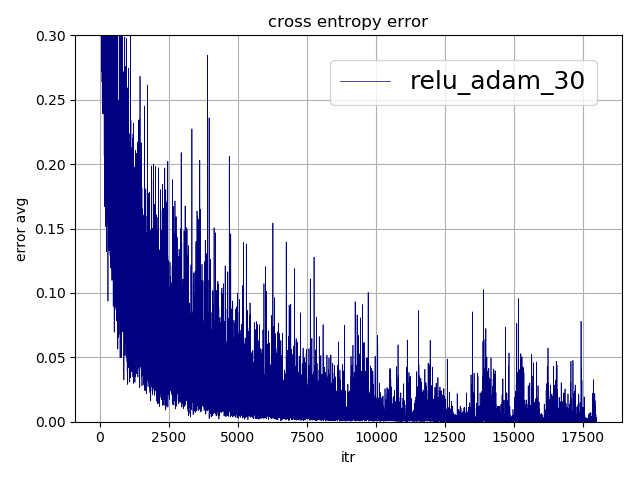
\includegraphics[clip, width=10.0cm]{./report_a4-5-1.png}
        \end{center}
      \end{minipage}
      \begin{minipage}{0.5\hsize}
        \begin{center}
          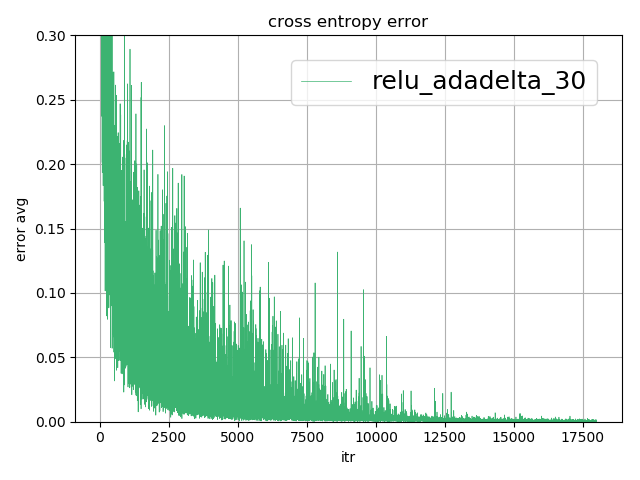
\includegraphics[clip, width=10.0cm]{./report_a4-5-2.png}
        \end{center}
      \end{minipage}
    \end{tabular}
    \caption{ Adam と AdaDelta の比較(左が Adam , 右が AdaDelta )}
    \label{fig-A4-5-1}
  \end{center}
\end{figure}

図\ref{fig-A4-5-1} の左側が最適化手法を Adam にしたもの、右側が AdaDelta にしたものである。図\ref{fig-A4-5-1} から学習速度は大きな差が見られないこと、AdaDelta の方が学習後半でのクロスエントロピー誤差の振幅が小さいことがわかる。Adam は AdaDelta の改良版ではあるが、学習対象によっては必ずしも Adam が最も学習効率が良いわけではないと考えられる。

\subsection*{A4 最適化手法の改良...比較}

学習用データで各最適化手法で 30 epoch 学習させた時の Accuracy をグラフ化したところ以下の図\ref{fig-A4-6-1}のようになった。図\ref{fig-A4-6-1} を見ると、RMSProp、AdaDelta、Adam の 3つの手法が学習が早く、それらに続いて Momentum SGD が学習が早かった。また、各最適化手法での最終的な Accuracy は表\ref{tableA4-6-1}のようになった。

\begin{table}[H]
\begin{center}
\caption{訓練データでの認識精度(最適化手法での比較)}
  \begin{tabular}{|c|c|} \hline
    最適化手法 & 認識精度  \\ \hline \hline
    SGD & 91.783 \% \\ \hline
    Momentum SGD & 97.250 \% \\ \hline
    AdaGrad & 91.458 \% \\ \hline
    RMSProp & 98.642 \% \\ \hline
    AdaDelta & 98.675 \% \\ \hline
    Adam & 98.592 \% \\ \hline
  \end{tabular}
	\label{tableA4-6-1}
\end{center}
\end{table}

\image{最適化手法の比較(学習用データの Accuracy)}{report_a4-6-1.png}{fig-A4-6-1}

次にテスト用データを用いて、バッチサイズ100、テスト回数100にして、発展課題A4 のそれぞれの最適化手法についてテストを行ったところ、認識精度は表\ref{tableA4-6-2} のようになった。

\begin{table}[H]
\begin{center}
\caption{テストデータでの認識精度(最適化手法での比較)}
  \begin{tabular}{|c|c|} \hline
    最適化手法 & 認識精度  \\ \hline \hline
    SGD & 95.12 \% \\ \hline
    Momentum SGD & 98.10 \% \\ \hline
    AdaGrad & 93.81 \% \\ \hline
    RMSProp & 98.05 \% \\ \hline
    AdaDelta & 98.29 \% \\ \hline
    Adam & 98.28 \% \\ \hline
  \end{tabular}
	\label{tableA4-6-2}
\end{center}
\end{table}

表\ref{tableA4-6-2}より、AdaGrad を除く全ての最適化手法において SGD よりも認識精度が高く、訓練用データに対して過学習せずに汎化性能が高められていると考えられる。

\subsection*{A5: カラー画像への拡張}

\subsubsection*{実装内容}

新たにカラー画像の学習用のプログラムファイル my\_nn\_color\_learn.py とテスト用プログラムファイル my\_nn\_color\_test.py を用意した。実装内容は以下の通りである。

\begin{itemize}
	\item モノクロ画像では Python3 系で学習させていたが、cPickle を用いるため Python2 系で実装を行った
	\item 次元数を $ d=1 \times 28 \times 28 $ から $ d=3 \times 32 \times 32 $ に変更
	\item 中間層のノード数を 1000 に変更
	\item 中間層の活性化関数は ReLU
	\item 逆伝播後の最適化手法は Adam を採用
	\item Adam のパラメータは $\alpha = 0.001, \beta_1 = 0.9, \beta_2 =  0.999, \epsilon = 10^{-8}$ に設定
\end{itemize}

学習方針としては、モノクロ画像と同じように、画像の左上から画素値を配列として扱っている。ただし今回はRGBの3チャンネルあるので、R の画素値 32 * 32 個、G の 画素値 32 * 32 個、B の画素値 32 * 32 個をこの順番で配列に 1列に格納して学習させる。

\subsubsection*{実行結果}

はじめに、訓練データ data\_batch\_1 を用いて、バッチサイズ 100、エポック数 300 にして学習を行った。横軸に学習回数、縦軸にクロスエントロピー誤差の平均値をとったグラフを以下の図\ref{fig-A5-1} に示す。

\image{学習経過とクロスエントロピー誤差の平均値(カラー画像)}{report_a5-1.png}{fig-A5-1}

また、横軸にエポック数、縦軸に訓練データに対するAccuracy をとったグラフを以下の図 \ref{fig-A5-2} に示す。

\image{学習経過と訓練データに対する認識精度(カラー画像)}{report_a5-2.png}{fig-A5-2}

図 \ref{fig-A5-1}、図 \ref{fig-A5-2} より、カラー画像におけるパラメータの学習がうまく進んでいることが確認できる。\\

次に、テストデータ 10000枚の画像について、学習したパラメータ(ファイル名は param\_color\_relu\_adam\_300.npz )を用いて、バッチサイズ 100、テスト回数100に設定して、テストデータに対する Accuracy を測定した。
テストデータにおける Accuracy と訓練データにおける Accuracy の値を以下の表 \ref{tableA5-1} に示す。
\begin{table}[H]
\begin{center}
\caption{認識精度(カラー画像)}
  \begin{tabular}{|c|c|c|} \hline
    テストデータ & 訓練データ & 差 \\ \hline \hline
    38.000 \% & 85.978 \% & 47.978 \%\\ \hline
  \end{tabular}
	\label{tableA5-1}
\end{center}
\end{table}

表 \ref{tableA5-1} から訓練データでは認識精度が高いが、テストデータに対してはかなり認識精度が低く、過学習が観測された。このような過学習は、訓練データのデータ数が少なく、かつ重みやバイアスの次元が高く、表現力が高いことや、畳み込み層やプーリング層のように画像の特徴量を抽出する層がないために発生したと考えられる。 

\end{document}
